\subsection{Growth diagrams for staircase tableaux}

In this section we set up the notation used in the remaining
sections. In particular, we slightly modify and generalise the
definition of $\Grm(\alt)$ from Section~\ref{sec:Stembridge}.
\begin{defi}
 For a pair of partitions $\wgt=(\pos\wgt,\neg\wgt)$, the partition
 $\pos\wgt$ is the \Dfn{positive part} and the partition $\neg\wgt$
 is the \Dfn{negative part}. Given an integer $n$ not smaller than
 the sum of the lengths of the two partitions,
 $[\pos\wgt,\neg\wgt]_n$ is the staircase
 \[
 ({\pos\wgt}{}_{,0},\pos\wgt{}_{,1},\dots,0,\dots,0,
 \dots,-\neg\wgt{}_{,1},-\neg\wgt{}_{,0}).
 \]

 A \Dfn{staircase tableau} is a sequence of staircases
 $\alt=(\wgt^0,\wgt^1,\dots,\wgt^r)$ such that $\wgt^i$ and
 $\wgt^{i+1}$ differ by a unit vector for $0\leq i<r$. If
 $\wgt^0=\emptyset$ the tableau is \Dfn{straight}, otherwise it is
 \Dfn{skew}. Unless explicitly stated, we consider only straight
 staircase tableaux.

 The \Dfn{extent}\footnote{It might be more logical to use \lq
 height\rq\ for the extent of a staircase, and \lq length\rq\ for
 the number $n$. However, Stembridge defines the height of a
 staircase as the number $n$. We therefore avoid the words \lq
 length\rq\ and \lq height\rq\ in the context of staircases
 altogether.} $\extent(\wgt)$ of a staircase
 $\wgt=[\pos\wgt,\neg\wgt]_n$ is the number of nonzero entries in
 $\wgt$. Put differently, the extent is the sum of the lengths of
 the partitions $\pos\wgt$ and $\neg\wgt$. The \Dfn{extent} of a
 staircase tableau is the maximal extent of its staircases.
\end{defi}

Given a staircase tableau we can create a growth diagram similar to
the procedure used in Section~\ref{sec:Stembridge}. However, it will
be convenient to label \emph{all} corners of the cells with
staircases, instead of labelling the corners which are not on the
main diagonal or first superdiagonal with a partition instead of a
staircase.
\begin{defi}
 The growth diagram \Dfn{$\Grm(\alt)$} corresponding to a (straight)
 staircase tableau $\alt$ is obtained in analogy to
 Definition~\ref{defn:P}: label the top-left corner with the
 staircase $\wgt^0$. If $\wgt^{i+1}$ is obtained from $\wgt^i$ by
 adding (respectively subtracting) a unit vector, $\wgt^{i+1}$
 labels the corner to the right of (respectively below) the corner
 labelled $\wgt^i$. \emph{All} the remaining corners of $\Grm(\alt)$
 are then labelled with staircases as follows. The positive parts
 on the corners to the left and below the path defined by the
 staircase tableau are obtained by applying the backward rule,
 whereas the forward rule determines the positive parts on the
 remaining corners. The negative parts are computed similarly.
\end{defi}
 
Alternatively, we can also create a growth diagram given a partial
filling and two partial standard Young tableaux.
\begin{defi}
 A \Dfn{partial filling} $\phi$ is a rectangular array of cells,
 where every row and every column contains at most one cell with a
 cross.

 Let $\phi$ be a partial filling having crosses in all rows except
 $\mathcal R$ (counted from the top), and in all columns except
 $\mathcal C$ (counted from the left). Let $P$ and $Q$ be partial
 standard Young tableaux having entries $\mathcal R$ and
 $\mathcal C$ respectively. Then the growth diagram
 \Dfn{$\Grm(\phi, P, Q)$} is obtained as follows. The sequence of
 partitions corresponding to $Q$ (respectively $P$) determines the
 positive (respectively negative) parts of the staircases on the
 bottom (respectively right) border. The remaining positive and
 negative parts are computed using the forward rule.

 If $\phi$ contains precisely one cross in every row and every
 column, we abbreviate $\Grm(\phi,\emptyset,\emptyset)$ to
 \Dfn{$\Grm(\phi)$}.
\end{defi}

Finally, any growth diagram in the sense above can be decomposed into
two classical growth diagrams, where all corners are labelled by
partitions.
\begin{defi}
 \Dfn{$\pos\Grm $} (respectively \Dfn{$\neg\Grm$}) denotes the
 (classical) growth diagrams obtained by ignoring the negative
 (respectively positive) parts of the staircases labelling the
 corners of a growth diagram $\Grm$.
\end{defi}
\begin{rema}
 The classical growth diagram associated to a (partial) filling $\phi$ is precisely $\pos\Grm(\phi, Q)$.
\end{rema}
\begin{rema}
 Two horizontally adjacent shapes in $\pos\Grm(\phi, Q)$ differ if and only if there is no cross above in this column. Two horizontally adjacent shapes in $\neg\Grm(\phi, Q)$ differ if and only if there is a cross above in this column.
\end{rema}
\begin{rema}\label{prop:transposed-growth}
 Transposing a filling $\phi$ is equivalent to interchanging $\pos\Grm(\phi)$ and $\neg\Grm(\phi)$.
\end{rema}

Finally, we introduce the operations on fillings we want to relate to promotion.
\begin{defi}
 Let $\phi$ be a filling of a square grid. The \Dfn{column rotation $\crot\phi$} (respectively, \Dfn{row rotation $\rrot\phi$}) of the filling $\phi$ is obtained from $\phi$ by removing the first column (respectively, row) and appending it at the right (respectively, bottom).

 The \Dfn{rotation $\rot\phi$} of a filling $\phi$ is $\crot\rrot\phi$.
\end{defi}

\subsection{Promotion and evacuation of alternating tableaux}
\label{sec:alternating}
In this section we prove Theorems~3.6
and~3.7, with the exception of
the case $n=2$.

Let us first recall a classical fact concerning the effect of
removing the first column of a filling on the growth diagram in terms
of Schützenberger's jeu de taquin.
\begin{prop}[\protect{\cite[A~1.2.10]{MR1676282}}]
 \label{prop:jdt-delete-column}
 Consider the classical growth diagrams $\Grm$ and $\half\Grm$ for the
 partial fillings $\phi$ and $\half\phi$, where $\half\phi$ is
 obtained from $\phi$ by deleting its first column. Let $Q$ and
 $\half Q$
 %
 be the partial standard Young tableaux corresponding to the
 sequence of partitions on the top borders
 %
 of the growth diagrams $\Grm$ and $\half\Grm$. Then
 $\half Q = \jdt Q$, the tableau obtained by applying
 Schützenberger's jeu de taquin to $Q$.
%
%
%
%
%
%
%
\end{prop}

The following central result connects the local rule for the symmetric group with column rotation, the operation of moving the first letter of a permutation to the end.
\begin{theo}\label{thm:growth-diagram-rotation}
 Let $\phi$ be a filling of an $r\times r$ square grid having
 exactly one cross in every row and in every column. Let $\lambda$
 and $\nu$ be two adjacent staircases in $\Grm(\phi)$, not on the left
 border of $\Grm(\phi)$, and $\lambda$ being to the left of $\nu$ or
 above $\nu$. Finally, let $\kappa$ and $\mu$ be the two
 corresponding staircases in $\Grm(\crot\phi)$, that is, the column
 index of $\kappa$ in $\Grm(\crot\phi)$ is one less than the column
 index of $\lambda$ in $\Grm(\phi)$. Then, provided that
 $n\geq\max(\extent(\kappa),\extent(\lambda),\extent(\mu),\extent(\nu))$,
 we have $\mu = \dom_{\fS_n}(\kappa+\nu-\lambda)$.
\end{theo}

Because the filling and the staircases of a growth diagram determine
each other uniquely, we immediately obtain the following corollary.
\begin{coro}\label{cor:growth-diagram-rotation}
 Let $\phi$ be a filling of an $r\times r$ square grid having
 exactly one cross in every row and in every column. Suppose that
 the staircases in $\alt=(1=\wgt^1,\dots,\wgt^{2r}=\emptyset)$ label
 a sequence of adjacent corners from the corner just to the right of
 the top-left corner to the bottom-right corner of $\Grm(\phi)$.
 Furthermore, suppose that the staircases
 $\half\alt=(\emptyset=\hm^0,\dots,\hm^{2r}=\emptyset)$ satisfy
 $\hm^i = \dom_{\fS_n}(\hm^{i-1}+\wgt^{i+1}-\wgt^i)$ for
 $i\leq 2r-1$. Then, provided that
 $n\geq\max(\extent(\alt),\extent(\half\alt))$, the filling of
 $\Grm(\half\alt)$ is $\crot\phi$.
%
%
\end{coro}
We remark that
%
Proposition~\ref{prop:jdt-delete-column}, restricted to permutations,
is a special case of Theorem~\ref{thm:growth-diagram-rotation}. More
precisely, it is obtained by considering the staircase tableau
$(1=\wgt^1,\dots,\wgt^{2r}=\emptyset)$ consisting of the partitions
labelling the corners along the top and the right border of a
classical growth diagram, with the empty shape in the top-left corner
removed.

It is not hard to extend the theorem to partial fillings; the
statement is completely analogous. Its proof proceeds by extending
the partial filling to a permutation. However, it turns out to be
more convenient to deduce the statements for staircase tableaux of
non-empty shape from the corresponding statements for staircase
tableaux of empty shape directly.

\begin{figure}[htb]
 \begin{enumerate}[(\alph{enumi})]
 \item\label{fig6_a}
 $\phi:$ \begin{tikzpicture}[baseline={([yshift=-.5ex]current bounding box.center)},scale=0.6]
 \node at (2.5,3) {$\lambda \text{ \raisebox{0.7mm}{\hbox to 1.5mm{\hrulefill}} } \nu$};%
%
 %
 %
 \node at (0.5,1.5) {\huge$\times$};
 \draw[-] (0,0) -- (0,4) -- (4,4) -- (4,0) -- (0,0);
 \end{tikzpicture} \quad $\crot\phi:$
 \begin{tikzpicture}[baseline={([yshift=-.5ex]current bounding box.center)},scale=0.6]
 \node at (1.5,3) {$\kappa \text{ \raisebox{0.7mm}{\hbox to 1.5mm{\hrulefill}} } \mu$};
%
%
%
 \node at (3.5,1.5) {\huge$\times$};
 \draw[-] (0,0) -- (0,4) -- (4,4) -- (4,0) -- (0,0);
 \end{tikzpicture}
 \begin{minipage}{3.8cm}
 $\pos\lambda=\pos\kappa+\square$\\
 $\extent(\pos\kappa+\pos\nu-\pos\lambda)\leq\extent(\pos\nu)$\\
 $\extent(\neg\kappa+\neg\nu-\neg\lambda)=\extent(\neg\nu)$
 \end{minipage}
 \[\pos\mu = \domS(\pos\kappa+\pos\nu-\pos\lambda),\quad \neg\lambda = \neg\kappa,\quad \neg\nu = \neg\mu\]


 \item\label{fig6_b} $\phi:$ \begin{tikzpicture}[baseline={([yshift=-.5ex]current bounding box.center)},scale=0.6]
 \node at (2.5,1) {$\lambda \text{ \raisebox{0.7mm}{\hbox to 1.5mm{\hrulefill}} } \nu$};%
%
%
%
 \node at (0.5,2.5) {\huge$\times$};
 \draw[-] (0,0) -- (0,4) -- (4,4) -- (4,0) -- (0,0);
 \end{tikzpicture} \quad $\crot\phi:$
 \begin{tikzpicture}[baseline={([yshift=-.5ex]current bounding box.center)},scale=0.6]
 \node at (1.5,0.85) {$\kappa \text{ \raisebox{0.7mm}{\hbox to 1.5mm{\hrulefill}} } \mu$};
%
%
%
 \node at (3.5,2.5) {\huge$\times$};
 \draw[-] (0,0) -- (0,4) -- (4,4) -- (4,0) -- (0,0);
 \end{tikzpicture}
 \begin{minipage}{3.8cm}
 $\neg\mu=\neg\nu+\square$\\
 $\extent(\neg\kappa+\neg\nu-\neg\mu)\leq\extent(\neg\kappa)$\\
 $\extent(\pos\kappa+\pos\nu-\pos\mu)=\extent(\pos\kappa)$
 \end{minipage}
 \[\neg\lambda = \domS(\neg\kappa+\neg\nu-\neg\mu),\quad \pos\lambda = \pos\kappa,\quad \pos\nu = \pos\mu\]


 \item\label{fig6_c} $\phi:$ \begin{tikzpicture}[baseline={([yshift=-.5ex]current bounding box.center)},scale=0.6]
 \node (la) at (3,3) {$\lambda$};
 \node (nu) at (3,2) {$\nu$};
 \draw[-] (la) -- (nu);
 \node at (0.5,1.5) {\huge$\times$};
 \draw[-] (0,0) -- (0,4) -- (4,4) -- (4,0) -- (0,0);
 \end{tikzpicture} \quad $\crot\phi:$
 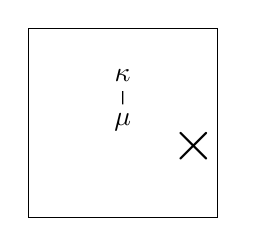
\begin{tikzpicture}[baseline={([yshift=-.5ex]current bounding box.center)},scale=0.6]
 \node (la) at (2,3) {$\kappa$};
 \node (nu) at (2,2) {$\mu$};
 \draw[-] (la) -- (nu);
 \node at (3.5,1.5) {\huge$\times$};
 \draw[-] (0,0) -- (0,4) -- (4,4) -- (4,0) -- (0,0);
 \end{tikzpicture}
 \begin{minipage}{3.8cm}
 $\pos\lambda=\pos\kappa+\square$\\
 $\extent(\pos\kappa+\pos\nu-\pos\lambda)\leq\extent(\pos\nu)$\\
 $\extent(\neg\kappa+\neg\nu-\neg\lambda)=\extent(\neg\nu)$
 \end{minipage}
 \[\pos\mu = \domS(\pos\kappa+\pos\nu-\pos\lambda),\quad \neg\lambda = \neg\kappa,\quad \neg\nu = \neg\mu\]

 \item\label{fig6_d} $\phi:$ \begin{tikzpicture}[baseline={([yshift=-.5ex]current bounding box.center)},scale=0.6]
 \node (la) at (3,2) {$\lambda$};
 \node (nu) at (3,1) {$\nu$};
 \draw[-] (la) -- (nu);
 \node at (0.5,2.5) {\huge$\times$};
 \draw[-] (0,0) -- (0,4) -- (4,4) -- (4,0) -- (0,0);
 \end{tikzpicture} \quad $\crot\phi:$
 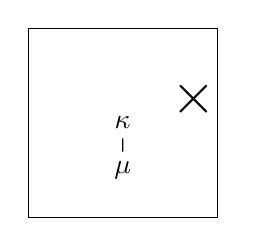
\begin{tikzpicture}[baseline={([yshift=-.5ex]current bounding box.center)},scale=0.6]
 \node (la) at (2,2) {$\kappa$};
 \node (nu) at (2,1) {$\mu$};
 \draw[-] (la) -- (nu);
 \node at (3.5,2.5) {\huge$\times$};
 \draw[-] (0,0) -- (0,4) -- (4,4) -- (4,0) -- (0,0);
 \end{tikzpicture}
 \begin{minipage}{3.8cm}
 $\neg\mu=\neg\nu+\square$\\
 $\extent(\neg\kappa+\neg\nu-\neg\mu)\leq\extent(\neg\kappa)$\\
 $\extent(\pos\kappa+\pos\nu-\pos\mu)=\extent(\pos\kappa)$
 \end{minipage}
 \[\neg\lambda = \domS(\neg\kappa+\neg\nu-\neg\mu),\quad \pos\lambda = \pos\kappa,\quad \pos\nu = \pos\mu\]

 \item\label{fig6_e} $\phi:$ \begin{tikzpicture}[baseline={([yshift=-.5ex]current bounding box.center)},scale=0.6]
 \node (la) at (3,2) {$\lambda$};
 \node (nu) at (3,1) {$\nu$};
 \draw[-] (la) -- (nu);
 \node at (0.5,1.5) {\huge$\times$};
 \draw[-] (0,0) -- (0,4) -- (4,4) -- (4,0) -- (0,0);
 \end{tikzpicture} \quad $\crot\phi:$
 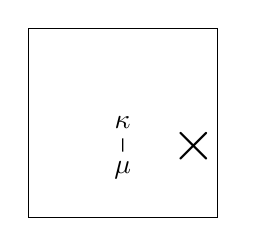
\begin{tikzpicture}[baseline={([yshift=-.5ex]current bounding box.center)},scale=0.6]
 \node (la) at (2,2) {$\kappa$};
 \node (nu) at (2,1) {$\mu$};
 \draw[-] (la) -- (nu);
 \node at (3.5,1.5) {\huge$\times$};
 \draw[-] (0,0) -- (0,4) -- (4,4) -- (4,0) -- (0,0);
 \end{tikzpicture}
 \[ \pos{\lambda'} - e_1 = \pos{\nu'} = \pos{\kappa'} = \pos{\mu'}, \quad \neg{\lambda'} = \neg{\nu'}= \neg{\kappa'} = \neg{\mu'} - e_1\]
 \end{enumerate}
 \caption{The cases considered in the proof of
 Theorem~\ref{thm:growth-diagram-rotation}.}
 \label{fig:different_cases_column_rotation}
\end{figure}
\begin{proof}[Proof of Theorem~\ref{thm:growth-diagram-rotation}]
 \textsc{Local rules for the positive and the negative parts.} 

 Let us first determine certain local rules satisfied separately by
 the positive and negative parts of the staircases $\kappa$,
 $\lambda$, $\mu$ and $\nu$. A summary of the various cases is
 displayed in Figure~\ref{fig:different_cases_column_rotation},
 where the rules we verify are displayed below the corresponding
 diagrams. In the following, addition and subtraction of integer
 partitions is defined by interpreting them as vectors in $\ZZ^n$.

\begin{enonce*}[remark]{\emph{First case, $\lambda$ left of $\nu$}} \ 

 Let
 $Q=(\emptyset=\mu_0, \mu_1, \ldots, \mu_{s-1} = \pos\lambda, \mu_s
 = \pos\nu)$
 be the partial standard Young tableau corresponding to the sequence
 of partitions in $\pos\Grm(\phi)$ on the same row as $\lambda$ and
 $\nu$, beginning at the left border. Let
 $\half Q = (\emptyset=\half\mu_0, \half\mu_1, \ldots,
 \half\mu_{s-2} = \pos\kappa, \half\mu_{s-1} = \pos\mu)$
 be the corresponding partial standard Young tableau in
 $\pos\Grm(\crot\phi)$.

 Suppose there is a cross in $\phi$ in the first column in a row
 below $\nu$, as in
 Figure~\ref{fig:different_cases_column_rotation}\ref{fig6_a}. Then, by
 Proposition~\ref{prop:jdt-delete-column}, $\half Q = \jdt Q$. This
 implies that the partitions
 $\mu_{s-1},\mu_s,\half\mu_{s-2},\half\mu_{s-1}$ satisfy the local
 (growth diagram) rule
 $\half\mu_{s-1} = \domS(\half\mu_{s-2}+\mu_s-\mu_{s-1})$, that is,
 $\pos\mu = \domS(\pos\kappa+\pos\nu-\pos\lambda)$. Moreover
 $\neg\kappa = \neg\lambda$ and $\neg\nu=\neg\mu$ because the growth
 for the negative parts of the staircases is from the top-right to
 the bottom-left.

 If there is a cross in the first column in a row above $\nu$, as in
 Figure~\ref{fig:different_cases_column_rotation}\ref{fig6_b}, we reason in a
 very similar way. In this case $\pos\kappa = \pos\lambda$ and
 $\pos\nu=\pos\mu$. For the negative parts of the staircases we
 consider the partial standard Young tableaux $Q$ and $\half Q$
 corresponding to the sequences of partitions beginning at the
 \emph{right} border of $\neg\Grm(\phi)$ and $\neg\Grm(\crot\phi)$
 respectively. We then have $Q = \jdt \half Q$ and conclude
 $\neg\lambda = \domS(\neg\kappa+\neg\nu-\neg\mu)$ as before, using
 the symmetry of the local rule, see
 Remark~\ref{rmk:symmetry-of-local-rule}.
\end{enonce*}

\begin{enonce*}[remark]{\emph{Second case, $\lambda$ above $\nu$}}\ 

 Depending on the position of the cross in the first column there
 are three slightly different cases, as illustrated in
 Figure~\ref{fig:different_cases_column_rotation}\ref{fig6_c},~\ref{fig6_d} and~\ref{fig6_e}.

\looseness-1
 Recall that the partitions on the right border of a (classical)
 growth diagram corresponding to the right to left reversal of a
 filling $\psi$ are obtained by transposing the partitions on the
 right border of the (classical) growth diagram corresponding to
 $\psi$. Consider now the filling $\psi$ below and to the left of
 $\lambda$, and let $\half\psi$ be the filling to the left and below
 $\kappa$. Note that the reversal of $\psi$ is obtained from the
 reversal of $\half\psi$ by appending the first column of $\psi$ to
 the right. We thus obtain that the transposes of the positive
 parts of the staircases $\kappa$, $\mu$, $\lambda$ and $\nu$
 satisfy the local (growth diagram) rule.

 The relation between the negative parts of the staircases $\kappa$,
 $\mu$, $\lambda$ and $\nu$ is obtained in a very similar way by
 considering the fillings above and to the right of $\nu$ and $\mu$.
\end{enonce*}

\noindent
\textsc{Bounding the extent and deducing the local rule.}\\*\vspace*{-1.1em}

 We now show
 $\mu = \dom_{\fS_n}(\kappa+\nu-\lambda)$, provided
 $n\geq\max(\extent(\kappa),\extent(\lambda),\extent(\mu),\extent(\nu))$.
 To do so, we extend the notion of extent to arbitrary vectors with
 all entries non-negative or all entries non-positive: for a vector
 $\pos\alpha\in\ZZ_{\geq0}^n$, the extent $\extent(\pos\alpha)$ is
 $n$ minus the number of trailing zeros. Similarly, for a vector
 $\neg\alpha\in\ZZ_{\leq0}^n$, the extent $\extent(\neg\alpha)$ is
 $n$ minus the number of leading zeros.

 The case illustrated in
 Figure~\ref{fig:different_cases_column_rotation}\ref{fig6_e} follows by
 direct inspection. We thus only consider the remaining four cases.
 Because $\pos\mu$ and $\neg\mu$ are obtained by sorting
 $\pos\kappa+\pos\nu-\pos\lambda$ and
 $\neg\kappa+\neg\nu-\neg\lambda$ respectively, the latter must have
 all entries non-negative. Similarly, also
 $\pos\kappa+\pos\nu-\pos\mu$ and $\neg\kappa+\neg\nu-\neg\mu$ have
 all entries non-negative, because $\pos\lambda$ and $\neg\lambda$
 are obtained by sorting these vectors, by the symmetry of the local
 rule, see Remark~\ref{rmk:symmetry-of-local-rule}.

 Suppose first that
 $n\geq\max(\extent(\kappa),\extent(\lambda),\extent(\nu))$. Then
 \[
 \dom_{\fS_n}(\kappa+\nu-\lambda)=\dom_{\fS_n}([\pos\kappa,\neg\kappa]_n+[\pos\nu,\neg\nu]_n-[\pos\lambda,\neg\lambda]_n)
 =\dom_{\fS_n}(\pos\alpha + \neg\alpha),
 \]
 where
 $\pos\alpha =
 [\pos\kappa,\emptyset]_n+[\pos\nu,\emptyset]_n-[\pos\lambda,\emptyset]_n$
 and
 $\neg\alpha=[\emptyset,\neg\kappa]_n+[\emptyset,\neg\nu]_n-[\emptyset,\neg\lambda]_n$.
 It remains to show that
 \[
 \extent(\pos\alpha) + \extent(\neg\alpha)
 =\extent\big(\pos\kappa+\pos\nu-\pos\lambda\big) +
 \extent\big(\neg\kappa+\neg\nu-\neg\lambda\big)\leq n,
 \]
 because then
 \begin{align*}
 \dom_{\fS_n}(\pos\alpha+\neg\alpha) &= [\domS(\pos\alpha),\domS(\neg\alpha)]_n\\
 &= [\domS(\pos\kappa+\pos\nu-\pos\lambda),
 \domS(\neg\kappa+\neg\nu-\neg\lambda)]_n = [\pos\mu,\neg\mu]_n =
 \mu.
 \end{align*}
 Similarly, suppose that
 $n\geq\max(\extent(\kappa),\extent(\mu),\extent(\nu))$. In this
 case, reasoning as above, we have to show that
 $\extent\big(\pos\kappa+\pos\nu-\pos\mu\big) +
 \extent\big(\neg\kappa+\neg\nu-\neg\mu\big)\leq n$.

 The first inequality is verified by inspection of
 Figure~\ref{fig:different_cases_column_rotation}\ref{fig6_a} and~\ref{fig6_c}, whereas
 the second concerns
 Figure~\ref{fig:different_cases_column_rotation}\ref{fig6_b} and~\ref{fig6_d}. Here we
 write, for example, $\pos\lambda=\pos\kappa+\square$ to indicate
 that the partition $\pos\lambda$ is obtained from the partition
 $\pos\kappa$ by adding a single cell, which implies the inequality
 for the extent.
\end{proof}
